\documentclass{article}

\usepackage[utf8]{inputenc}
\usepackage[T1]{fontenc}
\usepackage{hyperref}
\usepackage[french]{babel}
\usepackage{eurosym}
\usepackage{amsmath}
\usepackage{graphicx} % to include pictures
\usepackage{hyperref}
\usepackage{tcolorbox}
\usepackage{breqn}
\usepackage{amsfonts}

\title{INFO-F-302 Informatique Fondamentale\\ Projet : Problèmes de Satisfactions de Contraintes et Utilisation de l’Outil ChocoSolver}
\author{El Haman Abdeselam Abdeselam \and Minhas Prabhdeep}
\date{Année académique 2016-2017}

\begin{document}

\maketitle

\section{Problèmes d'échecs}

\subsection{CSP}
Les CSP pour les questions 1 et 2 se trouvent dans \textbf{quest1-2.pdf}.\\

Soient n, k1, k2 et k3 des entiers positifs.
Dans le problème d'échecs, nous considérons un échiquier de dimensions \textbf{n x n}, ainsi que \textbf{k1} tours, \textbf{k2} fous et \textbf{k3} cavaliers. 

Ces pièces ont une différente manière de se déplacer. Les tours peuvent aller verticalement ou horizontalement. Les fous, quant à eux, attaquent aux diagonales. Enfin, les cavaliers se déplacent en \textbf{L}, c’est-à-dire de deux cases dans une direction combinées avec une case perpendiculairement. \\

Nous pouvons compter deux problèmes dans les problèmes d'échecs, le problème d'indépendance ainsi que le problème de domination.
\begin{itemize}
\item Le problème d'indépendance consiste à déterminer s'il est possible d'assigner à chacune des pièces une position distincte sur l'échiquier de sorte qu'aucune pièce ne menace une autre pièce.
\item Le problème de domination consiste à déterminer s'il est possible d'assigner à chacune des pièces une position distincte sur l'échiquier de sorte que chaque case soit occupée ou menacée par au moins une pièce. 

De plus, nous ne considérons pas des pièces comme obtacles à d'autres pièces, c'est-à-dire que pour dominer une case, une pièce peut passer par dessus une autre.\\
\end{itemize}

Afin d'exprimer ces deux problèmes par un CSP équivalent, nous avons commencé par écrire les variables, le domaine ainsi que les notations utilisées dans les contraintes pour ceux-ci.

L'ensemble des variables est composé de toutes les coordonnées des pièces. Les tours sont notées $t_{i}$ et $t'_{i}$, les fous $f_{i}$ et $f'_{i}$ et finalement les cavaliers $h_{i}$ et $h'_{i}$.

Le domaine est compris entre \textbf{1} et \textbf{n}, \textbf{n} indiquant la taille de l'échiquier.

Pour les notations, nous avons la dimension de l'échiquier (n x n), ainsi que les notations pour représenter les différentes pièces (k1, k2, k3). 
De plus, \textbf{m} nous indique le nombre total de pièces que nous avons (k1 + k2 + k3). 
Enfin, \textbf{y} représente la suite de toutes les coordonnées des pièces, celles-ci sont alternées. Ainsi, les coordonnées x sont représentées sans les guillemets et les coordonnées y avec. Les \textbf{2 x k1} premières sont les tours, les \textbf{2 x k2} suivantes les fous et les \textbf{2 x k3} dernières les cavaliers.

\subsubsection{Question 1}
La première question nous demandait d'exprimer une instance quelconque du problème d'indépendance. L'ensemble des contraintes prend 4 contraintes pour ce problème.
$$C = \{c_{1} \cup c_{2} \cup c_{3} \cup c_{4}\} $$

$$c_{1} = ( y, \{ (v_{1}, ..., v_{2m}) \in  D^{2m} \mid \forall \hspace{0.1cm}  1\leq i \neq j \leq m, (v_{2i-1} \neq v_{2j-1}) \vee  (v_{2i} \neq v_{2j}) \} ) $$
La première contrainte nous indique que deux pièces ne peuvent pas se trouver au même endroit sur l'échiquier. 
Nous l'avons implémentée comme ceci, pour un ensemble \textbf{(v1, ..., v2m) $\in D^{2m}$}, il existe un \textbf{i} et \textbf{j}, différent et compris entre 1 et \textbf{m}, le nombre de pièce, tel que ces deux pièces ne peuvent pas avoir les mêmes coordonnées. 

L'ensemble est jusque \textbf{v2m} car dans y nous avons le nombre de pièce multipliées par 2, pour avoir toutes les coordonnées. De la même manière, nous multiplions les indices \textbf{i} et \textbf{j} par deux, car nous les avons bornés jusque \textbf{m}, et pour avoir la coordonnée y nous avons besoin de la valeur juste à cotée qui se trouve dans \textbf{y}. Pour rappel, dans \textbf{y}, par exemple pour la première tour, nous avions mis $t_{1}$, suivit de $t'{1}$, pour représenter ses coordonnées.\\

Pour les trois autres contraintes de ce problème, l'ensemble reste le même c'est seulement les conditions sur les deux pièces qui changent. \\

$$ c_{2} = ( y, \{ (v_{1}, ..., v_{2m}) \in  D^{2m} \mid \forall \hspace{0.1cm} 1\leq i \leq k_{1}, \forall \hspace{0.1cm} 1\leq j \leq m,$$
$$ (v_{2i-1} \neq v_{2j-1}) \wedge  (v_{2i} \neq v_{2j}) \} ) $$
La seconde contrainte se porte sur les tours, elle indique qu'aucune pièce ne peut se trouver sur l'horizontal ou la verticale d'une tour. Pour ceci, les bornes de \textbf{i} sont entre 1 et \textbf{k1}, afin de ne prendre en compte que les tours, et \textbf{j} se trouve entre 1 et \textbf{m}.  Ces deux pièces ne peuvent être à la même colonne et à la même ligne. 

  $$c_{3} = ( y, \{ (v_{1}, ..., v_{2m}) \in  D^{2m} \mid \forall \hspace{0.1cm}  k_{1}+1\leq i \leq k_{1}+k_{2}, \forall \hspace{0.1cm} 1\leq j \leq m, \forall \hspace{0.1cm} k \in \{-n, n \}, $$
  $$[ ((v_{2i-1} \neq v_{2j-1}+k) \vee  (v_{2i} \neq v_{2j}+k)) \wedge  ((v_{2i-1} \neq v_{2j-1}-k) \vee  (v_{2i} \neq v_{2j}+k)) ] \})$$
La troisième contrainte est sur la portée des fous, aucune pièce ne peut être sur les diagonales d'un fou. Pour cette contrainte, le \textbf{i} est entre \textbf{k1}+1 et \textbf{k1+k2}, afin de n'avoir que les fous, étant donné que les \textbf{k1} représentent les tours nous faisons un saut du nombre de tour présentes. Les bornes de \textbf{j}, par contre, restent les mêmes, de 1 à \textbf{m}. Dans cette contraintes, nous devons tenir en compte un autre indice qui définira les déplacements vers les diagonales, nous l'avons appelé \textbf{k} et celui-ci est compris entre \textbf{\{-n, n\}}.  Nous vérifions donc dans les 4 sens s'il n'y a pas d'autre pièces présentes.

 $$ c_{4} = ( y, \{ (v_{1}, ..., v_{2m}) \in  D^{2m} \mid \forall \hspace{0.1cm} k_{1}+k_{2}+1\leq i \leq m, \forall \hspace{0.1cm} 1\leq j \leq m,$$ $$\forall \hspace{0.1cm} k \in \{-2, 2\}, \forall \hspace{0.1cm}l \in \{-1, 1\},$$
  $$[((v_{2i-1} \neq v_{2j-1}+k) \vee  (v_{2i} \neq v_{2j}+l)) \wedge ((v_{2i-1} \neq v_{2j-1}+l) \vee  (v_{2i} \neq v_{2j}+k)) ] \})$$
Enfin, pour la dernière contrainte sur les cavaliers, nous devons vérifier qu'aucune pièce ne se trouve sur les déplacements en \textbf{L}. Pour cela, la borne inférieure de \textbf{i} est maintenant \textbf{k1+k2+1}, nous sautons donc toutes les tours et tous les fous. Et donc la borne supérieure est bien le nombre total de pièce : \textbf{m}. En plus de ceci, nous avons un \textbf{k} compris entre \textbf{\{-2, 2\}} et un \textbf{l} entre \textbf{\{-1, 1\}}, afin de pouvoir indiquer le déplacement vers une direction de deux cases suivit d'un mouvement perpendiculaire. 

\subsubsection{Question 2}
Une instance quelconque du problème domination devait être exprimée pour la seconde question. L'ensemble des contraintes est composé de 2 contraintes.
$$C = \{c_{1} \cup c_{2}\} $$

Où la première reste la même que pour la première question, 2 pièces ne peuvent pas être sur la même coordonnée dans l'échiquier.\\
$$c_{1} = ( y, \{ (v_{1}, ..., v_{2m}) \in  D^{2m} \mid \forall \hspace{0.1cm} 1\leq i \neq j \leq m, (v_{2i-1} \neq v_{2j-1}) \vee  (v_{2i} \neq v_{2j}) \} )$$ 

La deuxième contrainte indique qu'une pièce est soit :
\begin{itemize}
\item Occupée par une pièce
\item Menacée par une tour
\item Menacée par un fou
\item Menacée par un cavalier
\end{itemize}

$$c_{2} = (y, \forall \hspace{0.1cm} 1 \leq i \leq n, \forall \hspace{0.1cm} 1 \leq j \leq n,  u1_{i,j} \cup u2_{i,j} \cup u3_{i,j} \cup u4_{i,j})$$
    
Les indices \textbf{i} et \textbf{j} sont bornés entre 1 et \textbf{n}, nous les passons en paramètre aux 4 ensembles exprimant les conditions citées ci-dessus. 
\newpage
$$u1_{i,j} = \{(v_{1}, ..., v_{2m}) \in  D^{2m} \mid \exists k \in \{1, ..., m\}, v_{2k-1} = i \wedge v_{2k} = j\}$$
Le premier ensemble signifie que pour une case dont les coordonnées sont \textbf{\{i, j\}}, il existe une pièce quelconque ayant les même coordonnées.
L'indice \textbf{k}, appartenant à \textbf{\{1, m\}}, représente donc une pièce.

$$u2_{i,j} = \{(v_{1}, ..., v_{2m}) \in  D^{2m} \mid \exists k \in \{1, ..., k1\}, v_{2k-1} = i \vee v_{2k} = j\}$$
Dans le second ensemble, nous voulons qu'une tour aie la même ligne ou la même colonne que la case \textbf{\{i, j\}}. L'indice \textbf{k} symbolise les tours que nous avons, ses bornes étant entre 1 et \textbf{k1}.

$$u3_{i,j} = \{(v_{1}, ..., v_{2m}) \in  D^{2m} \mid \exists k \in \{k1+1, ..., k1+k2\}, p \in\{-n, n \},$$
$$ ((v_{2k-1} = i+p \wedge v_{2k} = j+p) \vee ((v_{2k-1} = i-p \wedge v_{2k} = j+p))) \}$$
De même le troisième ensemble indique qu'il existe un fou dans les diagonales d'une case \textbf{\{i, j\}}. Ici, vu que nous considérons les fous, les bornes de \textbf{k} sont comprises entre \textbf{k1+1} à \textbf{k1+k2}. Et comme pour la première question, nous devons intégrer un autre indice, que nous avons appelé ici \textbf{p}, afin de se déplacer dans les diagonales d'une case. 

$$u4_{i,j} = \{(v_{1}, ..., v_{2m}) \in  D^{2m} \mid \exists k \in \{k1+k2+1, ..., m\}, p \in \{-2, 2 \}, l \in \{-1, 1\},$$
 $$((v_{2k-1} = i+k \wedge v_{2k} = j+l)  \vee ((v_{2k-1} = i+l \wedge v_{2k} = j+k)))\}$$
Enfin le dernier ensemble exprime qu'il y a un cavalier aux déplacements \textbf{L} d'une case se trouvant aux indices \textbf{\{i, j\}}. Avec le même raisonnement qu'avant, les indices \textbf{k}, des cavaliers, sont compris entre \textbf{k1+k2+1} et \textbf{m}. De plus, pour faire les déplacements en \textbf{L} nous avons besoin de deux autres indices, appelés ici \textbf{p} et \textbf{l}.

\subsection{ChocoSolver}
La question 3 et la question bonus ont été implémentées dans le projet \textbf{CSPSolver}. 
\subsubsection{Question 3}
Cette question nous demande d'implémenter un programme qui, étant donné une instance du problème de domination ou d'indépendance, en calcule une solution à l'aide de ChocoSolver.\\

Un format d'entré et de sortie est fixé, où nous pouvons passer en paramètre les différentes options que nous voulons pour exécuter le programme. 
Afin de parser les arguments, nous avons utilisé la librairie Argparse4j. Pour cela, un fichier jar est donné qu'il faut rajouter dans le buildpath du projet en maven. 

Certains paramètres comme la dimension, le nombre de tours, cavaliers, fous, sont obligatoires. En ce qui concerne le type de problème demandé, nous vérifions qu'il y a bien qu'un seul paramètre entré, soit un \textbf{"-i"} (indépendance) soit un \textbf{"-d"}. \\

%model - piece - solveur
Une fois que tous les arguments sont initialisés, nous créons un Model ainsi que toutes les pièces demandées par l'utilisateur. Ensuite, pour ces pièces nous allons appliquer le code pour l'indépendance ou la domination. Et enfin, faire appel à \textbf{model.getSolver().findSolution()} afin de trouver notre solution.\\

%print
Afin d'afficher la solution, nous commencons par créer un tableau de dimension \textbf{n}. Puis, nous reprenons les positions x et y de toutes les pièces, ainsi que la première lettre de la pièce correspondante, et imprimons la solution. \\

%structure du code
Pour le projet, nous avons décidé de créer une structure générique, où nous avons les classes tour, fou et cavalier héritant d'une classe Pièce. 
Cette classe Pièce contient les méthodes que nous voulons implémenter pour tous les types de pièces existants, et nous permet de nous renvoyer les coordonnées x et y de celles-ci. De plus, dans cette classe nous avons créé une méthode qui, prenant en paramètre des coordonnées x et y, peut vérifier si une pièce y existe déjà. 

Les trois autres classes comportent les mêmes méthodes. Dans la première méthode, checkIndependency, nous vérifions qu'aucune pièce ne se trouve aux déplacements que peux effectuer la pièce en question. Cette fonction parcourt toutes les pièces, vérifie d'abord qu'aucune autre n'est présentes aux coordonnées x et y, puis applique les différentes contraintes que nous avons exprimée dans le CSP plus haut. Par exemple, pour les tours se serait vérifier qu'il n'y a aucune pièce ayant la même ligne ou colonne. 

La seconde méthode présente dans les 3 sous-classes, s'appelle inDomain, et prend en paramètre une case avec ses coordonnées. Elle nous renvoi, bien évidemment, le domaine tel que la case (x,y) se trouve dans le domaine de la pièce en question. Par exemple pour les fous, on vérifie pour les diagonales de cette case si une pièce fou s'y trouve.\\

%expliquer la domination
La résolution du problème de domination se fait comme suit: 
\begin{itemize}
\item Créer une liste de contraintes, everyConstraint
\item Vérifier qu'aucune pièce ne se trouve à cet endroit
\item Pour toutes les cases, créer une contrainte qui vérifie qu'elle se trouve dans le domaine d'une pièce, que ce soit une tour un fou ou un cavalier, ou qu'il y a une pièce présente à cette position.
\item Ajouter cette contrainte, dans la première liste de contraintes : everyConstraint
\item Dire au model de respecter toutes les contraintes pour toutes les cases
\end{itemize}

\subsubsection{Question bonus}
Pour la question bonus, nous avons créé une classe PieceGenerique qui, comme les fous, tours et cavaliers, hérite de la classe parent Pièce.\\

Nous représentons le domaine d'une pièce quelconque étant la fonction booléenne $\phi_{x,y} (i,j)$ qui
renvoit vrai ou faux si la case/pièce (i,j) est dominée par la case (x,y). C'est avec cette fonction
qu'on peut créer les contraintes de domination et indépendence pour une pièce quelconque tel que: \\

$$ c_{ind} = ( y, \{ (v_{1}, ..., v_{2m}) \in  D^{2m} \mid \forall \hspace{0.1cm} k_{1} + k_{2} + k_{3} \leq i \leq m, \forall \hspace{0.1cm} k_{1} + k_{2} + k_{3} \leq j \leq m,$$
$$ \neg \phi_ {v_{2i-1},v_{2i}} (v_{2j-1},v_{2j}) \} ) $$

$$ c_{dom} = ( y, \{ (v_{1}, ..., v_{2m}) \in  D^{2m} \mid \forall \hspace{0.1cm} 1\leq i \leq n, \forall \hspace{0.1cm} 1\leq j \leq n,$$
$$ (\exists k, \phi_{v_{2k-1},v_{2k}} (i,j) \hspace{0.1cm} \vee \hspace{0.1cm} (v_{2k-1} = i \wedge v_{2k} = j) \} ) $$


Nous demandons en arguments grâce au paramètre \textbf{"-g"} le nombre de pièce générique qu'un utilisateur demande. De plus nous avons défini le domaine d'une pièce avec des équations linéaires. Ces équations sont mises dans un fichier que l'utilisateur va mettre en paramètre grâce à \textbf{-file}. Les équations sont de la forme suivante : \textbf{a*x + b*y + c*i + d*j + e = 0}, l'opérateur peut bien sûr être autre qu'un \textbf{=} (>, >=, <, <=, !=). \textbf{x} et \textbf{y} représentent les coordonnées d'une pièce, et \textbf{i} et \textbf{j} celles de la pièce à dominer. Dans le fichier donné par l'utilisateur, le format est : a b c d e op., et nous supposons qu'il n'y a aucune erreur dans celui-ci. \\

Une fois que nous récupérons ces données, nous appliquons à la pieceGenerique le problème d'indépendance ou de domination. 

Nous avons utilisé le model.scalar() afin de pouvoir implémenter les contraintes des équations linéaires. Le model.scalar() nous permet en effet d'y mettre en paramètres une liste les IntVar, une liste des différentes varaibles \textbf{x},\textbf{y}, \textbf{i} et \textbf{j}, ainsi que l'opérateur, et le coefficient. Afin de respecter le format du model.scalar(), nous passons le coefficient de l'autre côté de l'équation, et donc le mettons en négatif.
	
\subsubsection{Question 4}
L'implémentation de cette question se trouve dans le projet \textbf{HorsemanMinimizer}. Le CSP s'y trouve dans le fichier \textbf{quest4.pdf}. \\

Pour ce problème, un entier n est passé en paramètre, qui indique la taille de l'échiquier. Il nous a été demandé de minimiser le nombre de cavaliers pouvant dominer l'échiquier. La sortie comprend le nombre minimum de cavaliers requit ainsi qu'un tableau affichant les positions de ces cavaliers sur l'échiquier.

Nous commençons par initialisé toutes les cases du tableau. Ensuite, nous vérifions que chaque case respecte bien la contrainte d'être soit dominée, soit occupée par un cavalier. 

L'ensemble des contraintes est défini comme ceci :  
  $$ C = (y, \{z \in D^{n^2} \hspace{0.1cm} | \hspace{0.1cm} \forall \hspace{0.1cm} 1 \leq i \leq n, \forall \hspace{0.1cm} 1 \leq j \leq n, \exists k \in \{2,-2\}, \exists l \in \{1,-1\},$$
 $$ a_{i+k,j+l}=1 \hspace{0.1cm} \vee \hspace{0.1cm} a_{i+l,j+k}=1 \hspace{0.1cm} \vee \hspace{0.1cm} a_{i,j)} = 1\}) $$ 
 
 Comme dans les premières questions, le \textbf{k} représente 2 déplacements d'un cavalier dans un sens, suivit d'un déplacement perpendiculaire exprimé par \textbf{l}. 
 
 Une fois que ces contraintes sont rajoutées dans le model, il faut minimiser le nombre de cavalier. Nous faisons d'abord la somme de chevaliers grâce au model.sum(). Puis, chocoSolver propose un model.setObjective(minimise), afin de minimiser le problème.\\
 
 Nous itérons le problème jusqu'à avoir la meilleure solution, et affichons toutes les possibilités.					
 
\section{Surveillance de musée}
Le code pour la dernière question, sur la surveillance de musée, se trouve dans \textbf{MuseumMonitorer}. Le CSP de cette question, quand à lui, est dans le fichier \textbf{musee.pdf}.\\

\subsection{CSP}
Pour les notations de ce problème, nous retrouvons : 
\begin{itemize}
\item n x n la dimension de l'échiquier
\item $a_{i,j}$ = case (i,j) du terrain (elle est égale à 1 si c'est un mur 0 sinon)
\item y variable représentant l'orientation des caméras
\item y' variables indiquant si une caméra est présente
\item z contient les valeurs de y
\item z' représentant les valeurs de y'
\item yy' = concaténation de y et y'
\item zz' = concaténation de z et z'\\
\end{itemize}

L'ensemble des variables est constitué de :
\begin{itemize}
\item Variables indiquant la direction de la caméra qui se trouve dans cette case
\item Variables par case indiquant que la case est occupée par une caméra\\
\end{itemize}

Le problème possède deux domaines, le premier comprenant toutes les directions qu'une caméra peut prendre, $D_1 = \{Nord, Sud, Est, Ouest, \emptyset\}$. 

Et le deuxième étant $D_2 = \{0,1\}$.

L'ensemble des contraintes est défini par l'union de 3 contraintes.
  $$c_{1} = ( yy', \{ vv' \in  D_1^{n^2} \times D_2^{n^2} \mid \forall \hspace{0.1cm} 1\leq i \leq n, \forall \hspace{0.1cm} 1\leq j \leq n,$$
  $$((v_{i,j} = \emptyset \hspace{0.1cm} \wedge \hspace{0.1cm} v'_{i,j} = 0)
   \hspace{0.1cm} \vee \hspace{0.1cm}
  (v_{i,j}  \neq \emptyset \hspace{0.1cm}\wedge \hspace{0.1cm} v_{i,j} = 1)) \} ) $$
Cette première contrainte, nous dit que $x'_{i,j} = 1$ ssi la caméra se trouve aux mêmes coordonnées. Nous avons les indices de \textbf{i} et \textbf{j} allant de 1 à \textbf{n}, la taille de l'échiquier, afin de prendre en considération toutes les cases de celui-ci. 

  $$c_{2} = ( y', \{ v' \in D_2^{n^2} \mid \forall \hspace{0.1cm} 1\leq i \leq n, \forall \hspace{0.1cm} 1\leq j \leq n, (a_{i,j} = 1 \wedge v'_{i,j} = 0 ) \vee (a_{i,j} = 0))$$  

La seconde contrainte permet de vérifier qu'une caméra ne se trouve pas dans un mur, ses coordonnées doivent être différentes d'un mu existant.

\begin{multline}
    c_{3} = ( yy',\hspace{0.1cm} \{ vv' |\hspace{0.1cm} \forall \hspace{0.1cm} 1\leq i \leq n, \forall \hspace{0.1cm} 1\leq j \leq n, \hspace{0.1cm} (a_{i,j}=1) \vee (v'_{i,j} = 1) \vee \\ \Bigg(a_{i,j} = 0\hspace{0.1cm} \bigwedge \hspace{0.1cm} \bigg(
    (\exists k \in \mathbb{Z} , (v_ {i+k,j} = Ouest \wedge (\forall 1 \leq l < k, v'_{i+l,j}=0
    \wedge a_{i+l,j}=0))) \\
    \bigvee \\
    (\exists k \in \mathbb{Z} , (v_ {i-k,j} = Est \wedge (\forall 1 \leq l < k, v'_{i-l,j}=0
    \wedge a_{i-l,j}=0))) \\
    \bigvee \\
    (\exists k \in \mathbb{Z} , (v_ {i,j+k} = Sud \wedge (\forall 1 \leq l < k, v'_{i,j+l}=0
    \wedge a_{i,j+l}=0))) \\
    \bigvee \\
    (\exists k \in \mathbb{Z} , (v_ {i,j-k} = Nord \wedge (\forall 1 \leq l < k, v'_{i,j-l}=0
    \wedge a_{i,j-l}=0))\bigg)
    \Bigg)\}
    )
  \end{multline}
  
  Enfin, la troisième et dernière contrainte exprime que chaque case doit être occupée par une caméra, ou être dominée par une caméra par le nord, le sud, l'est ou l'ouest.
  
  Le $(a_{i,j}) $ exprime la présence d'une caméra. Et comme on le voit, on vérifie pour chaque case dans ces 4 directions s'il y a une domination par une caméra.

\subsection{ChocoSolver}
L'utilisateur doit entrer en paramètre le nom du fichier dans lequel se trouve un tableau rectangulaire représentant la topologie de la salle à surveiller. 
Une case est soit vide, soit occupée par un obstacle. Un obstacle est symbolisé par \textbf{*}. De plus, les 4 murs sont toujours des obstacles. 
La sortie du code donne le nombre minimal de capteurs nécessaires, ainsi qu'un tableau montrant la position des caméras. \\

Dans l'implémentation du problème, nous commençons par parser le fichier mis en paramètre par l'utilisateur. Nous enregistrons dans une variable \textbf{murs}, contenant des booleans, le tableau. Nous travaillons avec des booleans, et donc s'il y a un obstacle a une position \{x, y\}, nous mettons le boolean à true, false sinon.Nous considérons qu'il n'y a pas d'erreurs dans le fichier mis e paramètre par l'utilisateur.\\

Nous devons donc minimiser le nombre de caméra présentes dans la pièce d'attente. Pour cela, nous devons respecter plusieurs contraintes. Premièrement, nous devons faire appliquer au model qu'une caméra existe seulement si son orientation n'est pas nulle, elle doit aller vers le nord, le sud, l'est ou l'ouest. Ensuite, il ne peut y avoir de caméra dans les murs, elles doivent être dans un espace vide. Finalement, chaque case doit être dominée ou occupée par une caméra. Afin de respecter cette dernière contrainte, pour chaque case nous vérifions pour ces 4 directions si une caméra y pointe.

Tout comme pour la question 4, nous itérerons toutes les solutions possibles jusqu'à avoir la meilleure.

\section{Résultats}
Nous avons créer des fichiers .jar afin de pouvoir exécuter les différentes implémentations.

\subsection{Exemples}
Voici quelques exemples:
\begin{itemize}
\item Problème d'indépendance avec un échiquier de dimension 5 x 5 , 3 tours, 2 fous ainsi que 2 cavaliers
 	\begin{center}
 		 	 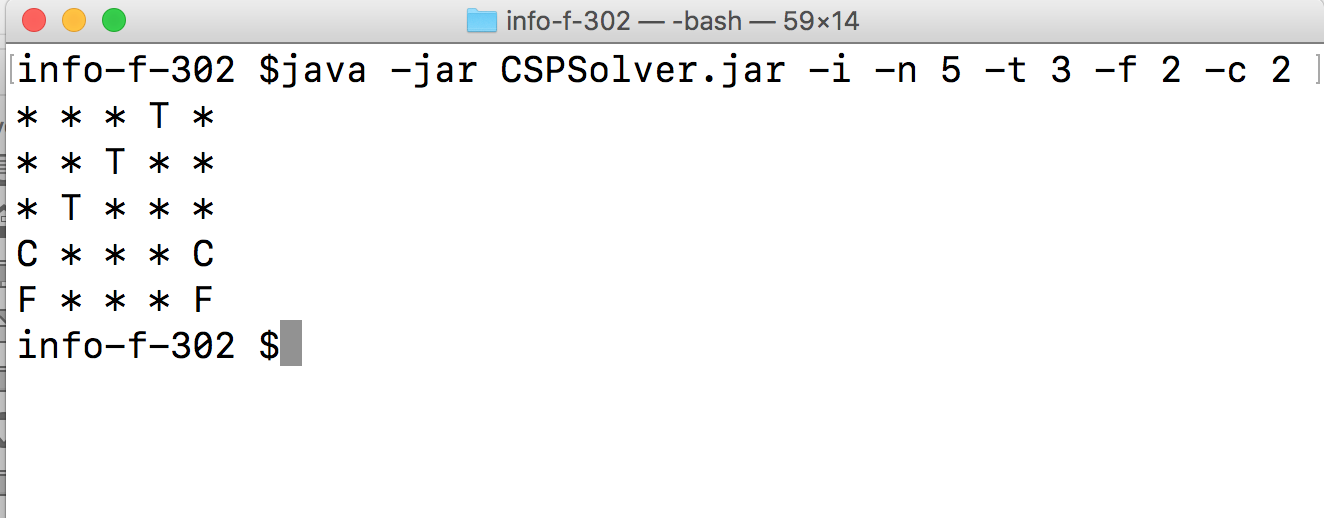
\includegraphics[width=75mm,scale=0.8]{./CSPindep.png}
 	\end{center}
\item Problème de domination avec un échiquier de dimension 4 x 4 , 2 tours, 1 fous ainsi que 2 cavaliers
 	\begin{center}
 		 	 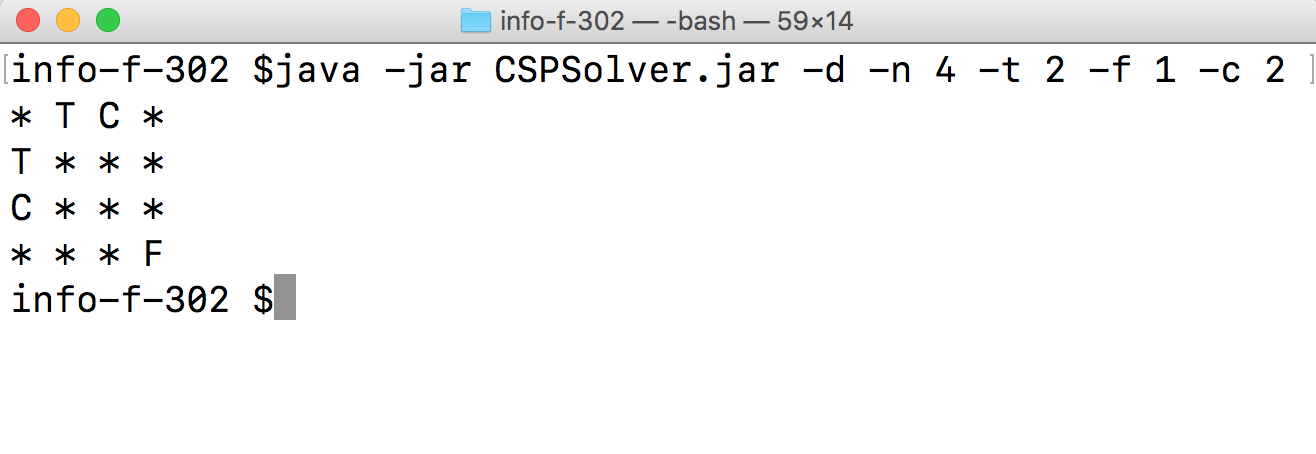
\includegraphics[width=75mm,scale=0.8]{./CSPdep.png}
 	\end{center}
\item Une implémentation de la question bonus, pour le problème d'indépendance, avec un échiquier de dimension 5 x 5 , 2 tours, 1 fous, 2 cavaliers et 2 pièces génriques. Les équations linéaires de ces pièces génériques se trouvent dans le fichier pieceGen.txt.
 	\begin{center}
 		 	 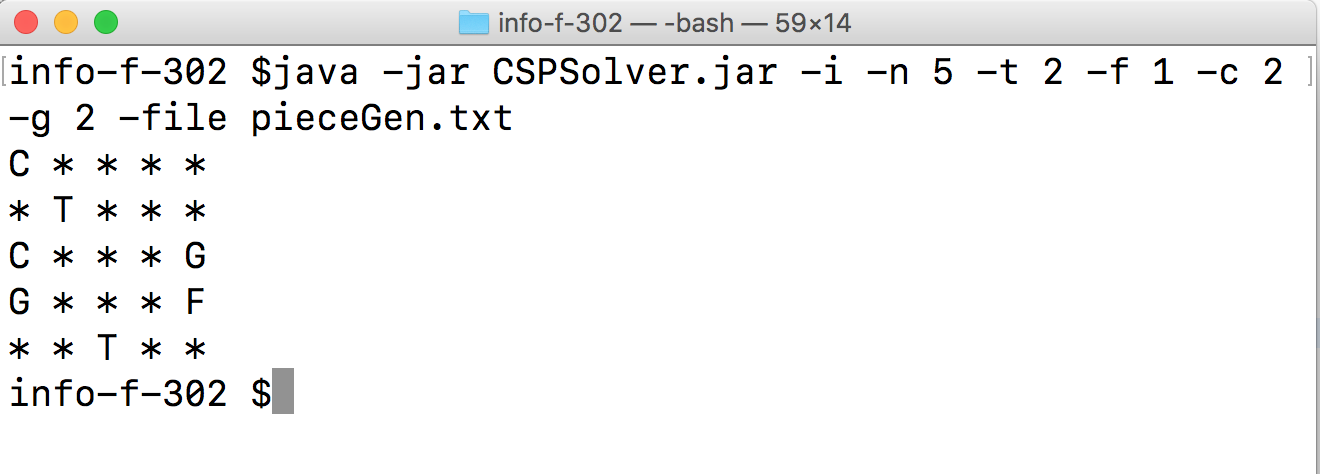
\includegraphics[width=75mm,scale=0.8]{./CSPgen.png}
 	\end{center}
 	\begin{itemize}
 	\item Le fichier pieceGen.txt fournit par l'utilisateur prend cette forme :
 	 	\begin{center}
 		 	 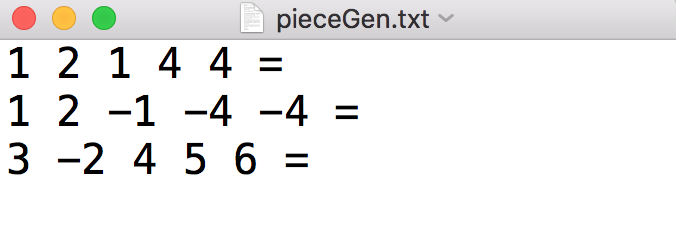
\includegraphics[width=75mm,scale=0.8]{./pieceGen.png}
 	\end{center}
 	\end{itemize}
\item Pour la question4, minimisation des cavaliers, nous devons entrer en paramètre la taille de l'échiquier.
 	\begin{center}
 		 	 \includegraphics[width=75mm,scale=0.8]{./Horsemin.png}
 	\end{center}`
\item La dernière question prend en paramètre le nom du fichier contenant l'échiquier. Le code renvoie affiche toute   les solutions jusqu'à atteindre l'optimale, celle qui utilise le moins de caméra. 
 	\begin{center}
 		 	 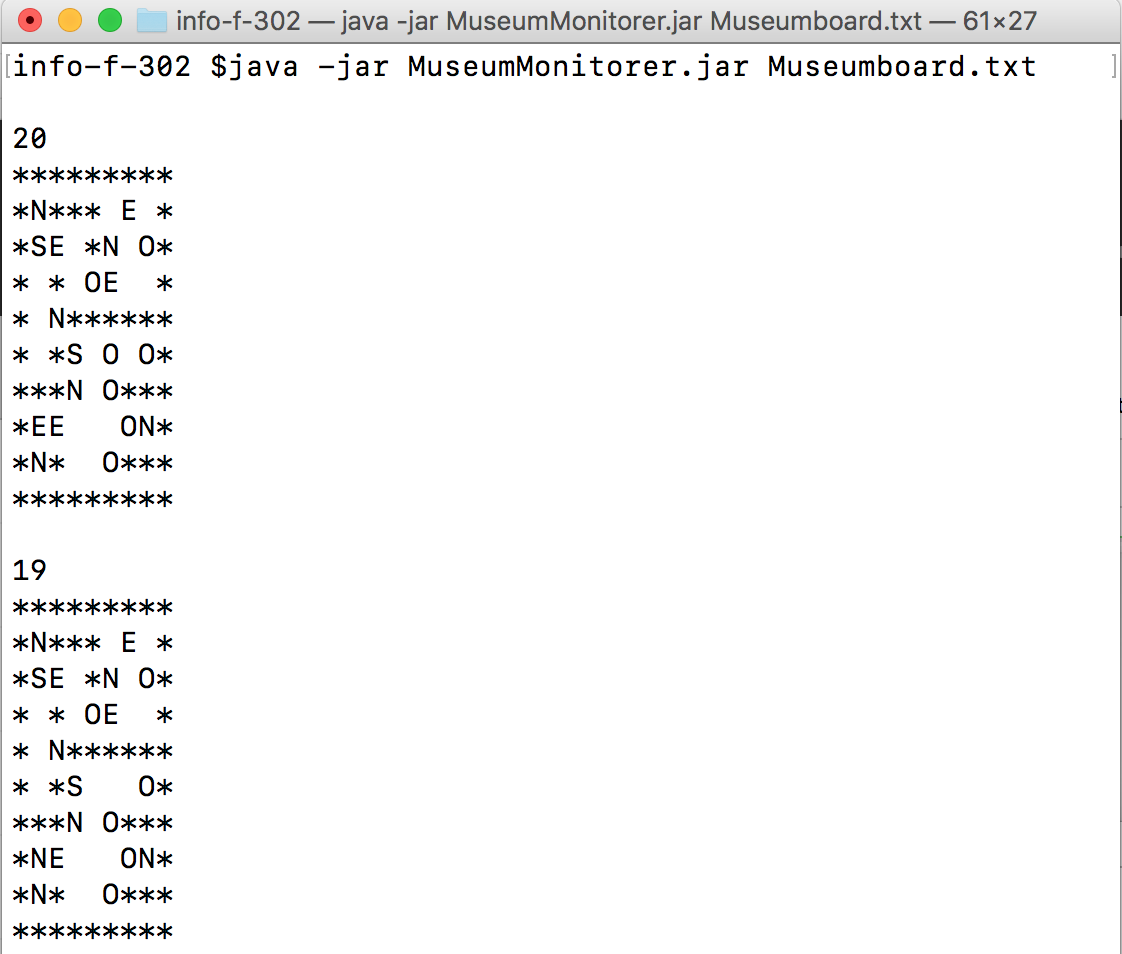
\includegraphics[width=75mm,scale=0.8]{./musee1.png}
 	\end{center}
 	\begin{center}
 		 	 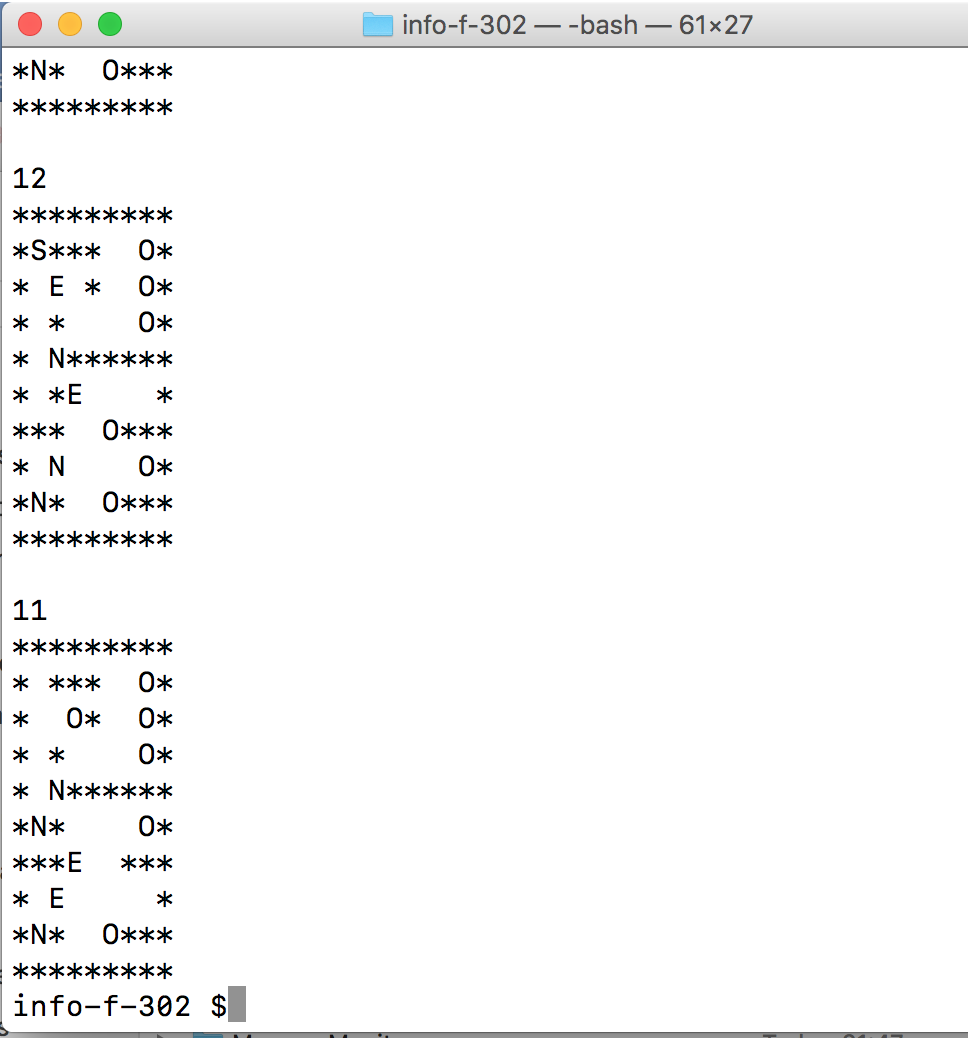
\includegraphics[width=75mm,scale=0.8]{./musee2.png}
 	\end{center}
\end{itemize}

\end{document}